% This is samplepaper.tex, a sample chapter demonstrating the
% LLNCS macro package for Springer Computer Science proceedings;
% Version 2.20 of 2017/10/04
%
\documentclass[runningheads]{llncs}
%
\usepackage{graphicx}
\usepackage{amssymb}
\usepackage{amsmath}
\usepackage{mathtools}
\usepackage{xurl}

% Used for displaying a sample figure. If possible, figure files should
% be included in EPS format.
%
% If you use the hyperref package, please uncomment the following line
% to display URLs in blue roman font according to Springer's eBook style:
% \renewcommand\UrlFont{\color{blue}\rmfamily}

\begin{document}
%
\title{Blockchain Cohomology\thanks{Supported by Constellation Labs}}
%
%\titlerunning{Abbreviated paper title}
% If the paper title is too long for the running head, you can set
% an abbreviated paper title here
%
\author{Wyatt Meldman-Floch\inst{1}\orcidID{0000-0001-6582-5925} }
%
\authorrunning{W. Meldman-Floch}
% First names are abbreviated in the running head.
% If there are more than two authors, 'et al.' is used.
%
\institute{Constellation Labs, San Francisco CA 94108, USA }
%
\maketitle              % typeset the header of the contribution
%
\begin{abstract}
The following explores topological models of distributed computing for scalability focused Blockchain technologies. Applications of these models are provided in terms of emerging Blockchain protocols and scalability approaches as well as programming models allowing type-level verification.
\keywords{Distributed computing \and Homology \and Algebraic topology}
\end{abstract}
%
%
%
\section{Introduction} 
Existing models of blockchain technology are being expanded to incorporate scalability advancements in distributed computing. However, despite their compatibility, these new approaches lack verification methods common in large scale data processing. By connecting topological models of distributed computing to scalable distributed architectures using Homotopy type theory, we create a hybrid topological model applicable to common architectures in Big Data and emerging scalable blockchain technology. Applications are provided across common scalable architectures in distributed computing that are being adopted by new blockchain technology.

\subsection{Related Work}
The following is a literature overview of references used in formulating this work's main results, from a historical perspective. 

\subsubsection{Topological Models in Distributed Computing}
Topology is a mathematical field focused on higher dimensional connective properties of algebraic objects. In the context of distributed computing, these objects are generalizations of graphs, and their connectivity properties related to the computability of distributed algorithms. Exploiting certain topological properties of higher dimensional geometric objects to prove results of distributed algorithms is referred to as the topological approach to distributed computing. Techniques from combinatorial and algebraic topology have advanced characterization of synchronous and asynchronous distributed algorithms as well as their solvability~\cite{ref_article1,ref_article2,ref_article3,ref_article4}. 

The first applications of topology to distributed computing were in deriving the lower bounds for solving the distributed set agreement~\cite{ref_article12}, which introduced a new paradigm based on algebraic topology for reasoning about asynchronous computations, where at-most one process can fail. The framework consisted of modeling tasks and protocols as simplicial complexes, and applied homology~\cite{ref_article5,ref_article9} theory to reason about them. A key feature in this framework is that the exponential number of possible executions can be compactly represented using a static topological object in a model independent manner. In certain systems, such as those explored below relating to blockhain technology and scalability, the simplicial complexes are manifolds~\cite{ref_article6,ref_article7,ref_article8}, a special class of simplicial complexes that are intuitive due to their geometric nature. The application of homology theory in these models forms a direct connection to Homotopy type theory~\cite{ref_article9,ref_article10}, the basis for modern static analysis in software engineering as well as in programmatic proof assistants. This connection is realized by a result known as the Curry-Howard correspondence which is an isomorphism between mathematical proofs and programs. This correspondence allows us to verify programs at compile time, given a type system and typesafe (type preserving) implementation, as is enforced by the functional programming paradigm.

\subsubsection{Homotopy Type Theory and Verification}
Homotopy type theory is an interpretation of constructive type theory that connects logic and topology~\cite{ref_book1}. Specifically, Homotopy theory is a tool for constructing models of systems of logic and constructive type theory is a formal calculus for reasoning about homotopy. Computational implementation of type theory allows computer verified proofs in homotopy theory and is the formalism from which static analysis and functional programming emerged from~\cite{ref_article10}.

Proof assistants and type systems are explicit examples of tools for proofs or programs for which compilation verifies correctness. Their use in mathematics and computer science is increasingly common for managing complex proofs and programs. Examples of the success of proof assistants and type systems respectively include the proof of the Four Color Theorem and the Feit-Thompson Odd-Order Theorem, as well as large pieces of software such as a C compiler and the Standard ML programming language. Homotopy type theory is used in strongly typed programming languages like C and functional languages like Haskell to provide compile time verification. The ability to verify a program, especially all aspects of a distributed system before deployment, has been a fundamental advantage that ushered the emergence of Big Data over the last ten years.

\subsubsection{Functional Programming and Big Data}
Big Data~\cite{ref_article11,ref_book2} refers to applications pertaining to data sets so big that distributing the processing is not an optimization but a fundamental requirement. Given the exponentially increasing amount of data generated by human information systems, the field continues to grow. It is widely held that the advent of Big Data stems from the MapReduce white paper~\cite{ref_proc1}, which introduced the first programming model strictly designed for processing and generating large, inherently distributed, datasets. 

A programming model is the style and interface used for development and the leading programming model in Big Data, MapReduce, is fundamentally a functional programming model as it is just the combination of $.map()$ and $.reduce()$ operators, which are by definition declarative functional operations on collections. Functional, as opposed to procedural, programming is a paradigm in software engineering that simplifies verification and improves visibility in distributed processes due to statelessness~\cite{ref_book3}. If something fails during state transformations developers have to recompile and redeploy their source code, restarting a workflow from scratch. The reason why functional languages encourage scalable software architectures is because of the fact that they eliminate as much shared state as possible from a language. This leads to scalable micro-services or components and these micro-services then scale naturally into larger components.

\subsubsection{Blockchain Technology and Scalability}
The first Blockchain was formulated roughly 30 years ago as a way to time-stamp digital documents~\cite{ref_article13}. At its core a Blockchain is an application of a distributed consensus algorithm operating on cryptographically signed data to form a secure append only log; secure in the sense that forgery is computationally intractable. Lately blockchain technology has become popular due to its application in creating cryptocurrencies like Bitcoin, but wider applications in verifiable decentralized code execution (provided by Smart Contract platforms like the Ethereum protocol) and open network security (provide by the Constellation protocol) have emerged. 

A major limitation in adoption of blockchain applications is an inherent scalability issue due to the fact that traditional Byzantine Fault Tolerant consensus algorithms require serial execution across a distributed system, making concurrency difficult or impossible. New parallelizable consensus algorithms and system architectures have emerged however, based on the design of highly concurrent and distributed data processing tools common in Big Data. These new approaches~\cite{ref_url3,ref_url6} lack formal verification methods employed by similar tools in both blockchain and the Big Data space however, the creation of which is the focus of the models constructed below.

\section{Consensus Protocols}
Recent advancements in distributed computing have adopted methods from algebraic topology to formally define consensus protocols~\cite{ref_article1,ref_article2}. First define an execution space as a topological space equipped with a discrete product topology~\cite{ref_article3}. Defining a distributed process in terms of topology only requires us to care about the structure of the set of possible schedules of a distributed system ~\cite{ref_article4}. By defining an execution space in terms of the homology of Protocol Complexes ~\cite{ref_article2}, define a Protocol Complex $S_k: P_k{\Delta^q}$ as the q-dimensional standard simplex
\begin{equation}
\Delta^q = \{x \in \mathbb{R} | \Sigma x_j = 1, x_j \geq \forall j \}
\end{equation} 
at morphism $k$ described by the following vertex set
\begin{equation}
S_k = \{v_{i,0} \dots v_{i,q}\}
\end{equation}
where $P \subset S$ is the set of all admissible configurations and $S$ is the set of all possible configurations.

Define a consensus protocol $P^\sigma_{*}(S):\{S_k, \partial_k\}$ as the singular homology of a simplicial chain complex, carried by a group morphism implementing distributed consensus. Let $S_k$ be a simplex configuration at step $k$ and $\partial_k$ be the differential of a distributed consensus morphism:
\begin{equation}
P^\sigma_{*}(S): 0 \leftarrow \dots P^\sigma(S_{k-1})\xleftarrow {\partial_{k-1}} P^\sigma(S_{k})\xleftarrow {\partial_{k}} P^\sigma(S_{k+1}) \dots
\end{equation}
where $P_k = ker \partial_k / im \partial_{k+1}$ and is also an abelian group. Thus, $P_*= (P_k) \ | k \in \mathbb{Z}$ is a graded abelian group which is referred to as the homology of a Protocol Complex $S$. We abuse our notation of $P$ but rectify by noting that an admissible state $k$ is required for anther step $k + 1$, thus we define $P$ as the functor carrying our consensus operator defined below.

Define a consensus operator $\sigma$ as the group morphism on the singular q-simplex $\sigma: \Delta^q \rightarrow S$ 
\begin{equation} \label{eq1}
\sigma_k: S_{k-1} \times P_k \rightarrow S_{k}
\end{equation} \label{eq1}
which are continuous on discrete topologies such as $\Delta^q$ \cite{ref_article1}. Define homology between configurations as a measure of divergence given by the differential 
\begin{equation} 
\partial(\sigma) = \sum^{q+1}_{i=1} (-1)^{i-1}(\sigma \circ \delta_q^{i} )
\end{equation}
for continuous functions $\delta^{i}_q: \Delta^{q-1} \rightarrow \Delta^q | 1 \leq i \leq q+1$ where 
\begin{equation}
\delta^{i}_q(x_1, \dots, x_q) = (x_1, \dots x_{i-1}, 0, x_i, x_{i+1}, \dots, x_{q-1}, \dots, x_q)
\end{equation}

As the graded abelian group of our Protocol Complex is the simplicial singular homology group and $\sigma$ is our homology preserving map, it is trivial to note that homology holds $\forall k \in \mathbb{Z}$, i.e.
\begin{equation} \label{eq1}
\partial_k \circ \partial_{k+1} = 0
\end{equation} \label{eq1}
As a corollary of the fact that the geometric realization of a simplicial complex is dually a topological space, due to the vanishing homology up to $k$, $P_k\Delta^q$ is k-acyclic, or that there is a consistently forward moving "arrow of time".

\subsection{Protocol Topologies}
It's possible to layer Protocol Complexes defined as above with guarantees about consistency as long as continuity is preserved. Our definition of homology above is verification criteria for the ability to exchange configuration states between Protocol Complexes.

Specifically, a valid 'layering' as the existence of a functoral vertex map between singular homologies (defined equivalently here as the disjoint subset of Protocol Complexes) $l: \bigcup_{k} P_{\pi} \rightarrow \bigcup_{k} P_{\pi+1}$.

Making use of Homotopy type theory allows us to focus on structure by treating topological characteristics called homotopy groups as primitives. Noting that simplicial complexes together with simplicial vertex maps form a category, if we redefine our k-acyclic distributed consensus protocol $\sigma$ categorically as the functoral carrier $\Sigma_{*}$  we can form a chain complex that adheres to the homology theory of homotopy types ~\cite{ref_article5}.

Let us define a 'layering' as a Protocol Topology $T^{\Sigma}_P: $ $\Sigma_{*}P_\pi$, the singular homology of a chain complex of Protocol Complexes carried by a homotopy preserving functor $\Sigma_*$. The Protocol Topology is given by the following chain complex

\begin{equation}
T^{\Sigma}_P: 0 \leftarrow \Sigma_{*}P_\pi \xleftarrow{\partial} \Sigma P_{0} \xleftarrow{\partial} \dots \Sigma P_i \ | i \leq \pi \in \mathbb{Z}
\end{equation}
where $\Sigma_\pi: $ $ker \partial^{\pi}_{k}/im \partial^{\pi}_{k+1} \rightarrow \partial^{\pi+1}_{k} /im \partial^{\pi+1}_{k+1}$ 

For Protocol Complex morphisms $\Sigma_\pi, \Sigma_{\pi+1}$ chain homotopy from $\Sigma_\pi$ to $\Sigma_{\pi+1}$ is a homotopy preserving graded abelian group morphism $l: P_{\pi} \rightarrow P_{\pi+1}$ yielding a vanishing homology, i.e. 

\begin{equation}
\begin{split}
\Sigma_\pi - \Sigma_{\pi+1} =  \partial^{\pi}\circ l + l \circ \partial^{\pi+1} \\
= \partial^\pi \circ \partial^{\pi+1} = 0 \\
\end{split}
\end{equation}
Noting that these conditions are met by the definitions of an acyclic carrier as above, it follows that a Protocol Topology as defined above is $\pi$-acyclic.
 
\subsection{Applications: Scale out Networking}
Traditional Blockchains have come up short in their ability to support real world use cases, mainly due to scalability issues. In terms of scalability, sharding or partitioned approaches have taken form in improvements to Bitcoin with Lightning~\cite{ref_url4} as well as base layer protocols like Zilliqa~\cite{ref_url5}. In these approaches, relays or subnets are deployed to ferry larger amounts of transactions into a fixed-size configuration state (block). The key to their success is the application of Scale Out Networking~\cite{ref_article11}, adding another layer to the network topology to buffer and compress data which results in faster routing and query times. If we consider either base layer protocol as a Protocol Complex, then a partitioned or sharding mechanism is described by our model of Protocol Topology. A type hierarchy is enough to verify a protocol's equivalence to a Protocol Topology due to covariance, which is a valid null differential as detailed by R. Grahm above. Specifically, given a base layer protocol $\Sigma_\pi$ with block type $\pi$, a type preserving operation $\Sigma_{\pi+1}$ such as a buffering service in a multi layered (in this case L2) topology, then if there exists covariance between their data types $\pi$, $\pi+1$ then $\partial^\pi \circ \partial^{\pi+1} = 0$. Specifically, consider a protocol with an L2 topology:
\begin{equation}
T^{\Sigma}_P: 0 \leftarrow \Sigma_{*}P_\pi \xleftarrow{\partial} \Sigma P_{0} \xleftarrow{\partial} \Sigma P_2 \ 
\end{equation}
This Protocol Topology is a corresponding model to an L2 system architecture (see Fig.~\ref{fig1}). A program implementing the above protocol is verifiable by ensuring functoral covariant state transitions which can be enforced by static analysis~\cite{ref_article10} (type checking at compile time).
\begin{figure}
\centering
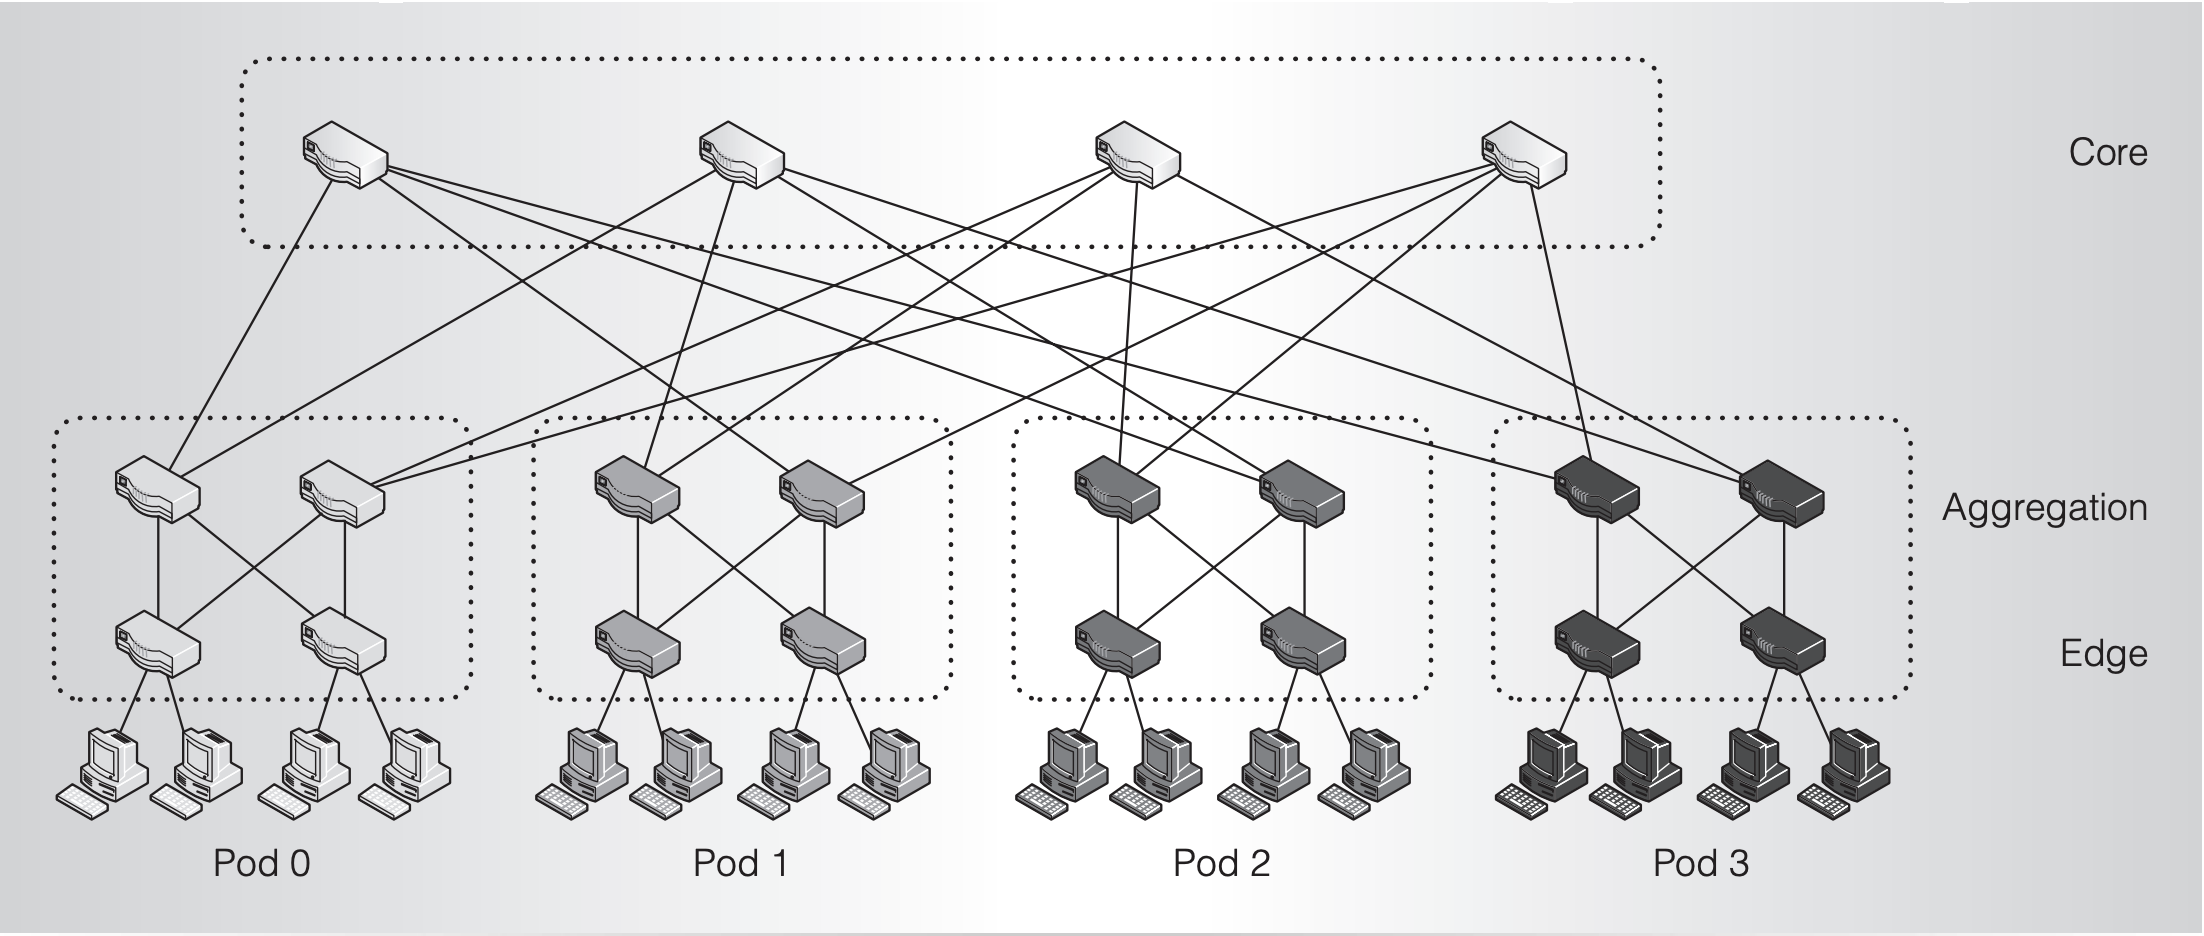
\includegraphics[width=0.6\columnwidth]{l2-system-architecture.png}
\caption{System architecture diagram of an L2 system ~\cite{ref_article11}} \label{fig1}
\end{figure}

\section{Blockchain Cohomology}
Distributed architectures designed topologically can be verified at the type level. In order to model distributed state, we need to design our topologies such that data locality, or the logic behind the distribution of data in distributed database is mathematically tractable. We introduce methods from Abstract Differential Geometry, namely finitary cech-deRham cohomology in order to define an orientable manifold from our definition of Protocol Topology.

\subsection{Block Sheaves}
First we need to introduce the dual of homology as described above, namely cohomology. In describing our Protocol Complex it only makes sense to have an arrow moving 'forward in time' as consensus itself is acyclic, with each iteration pointing 'backwards in time' to its previous state. In this sense our evolution was the compounding dimensionality of the space of all configurations, as implied by the discrete product topology of a Protocol Complex. In defining an orientable manifold, we need to move 'backwards' through our space, i.e. from higher to lower dimension. This is shown as the differential on an arrow going right instead of left. 

In principle, Abstract Differential Geometry (ADT) admits any topological space as a base space on which to 'solder sheaves' for carrying out differential geometry~\cite{ref_article6}. i.e. constructing a manifold. By constructing the Protocol Topology within a monoidal category, A. Malios et al. showed that the singular cohomology of a Protocol Topology is equivalent to an A-module of Z+-graded discrete differential forms, otherwise known as discrete differential manifolds. This forms an execution tree, a sequence of configurations in a poset (directed acyclic graph) topology. A decision tree can be assigned to any set of executions that captures the decision of choosing a successive configuration. A Blockchain can be defined as an extension of an execution tree, where each block is formulated as a sheaf with a well defined tensor operation and each successive block verified by a decision tree. We define a sheaf $\epsilon$ as the 'enrichment' of any cochain $\mathbb{A}$-complex of positive degree/grade, corresponding to the $\mathbb{A}$-resolution of an abstract $\mathbb{A}$-module
\begin{equation}
S^*: 0 \rightarrow \epsilon \rightarrow S^0 \xrightarrow{d^0} S^1 \xrightarrow{d^1} \dots
\end{equation}
and homomorphism given by Cartan-Kahler-type of nilpotent differential operator d. We will make use of the fact that an $\mathbb{A}$-module sheaf $\epsilon$ on any arbitrary topological space (shown above with an arbitrary simplicial cochain-complex) admits an injective resolution.

Blockchains are naturally equipped with a sheaf, known as a block hash, which contains topological state data about the configuration of the system. Every abelian unital ring (of which this sheaf theortic construction derives from) admits a derivation map~\cite{ref_article7}, allowing us to 'unpack' data within a block recursively under the product operation. By noting the equivalence of Sorkin's fintoposets to simplicial complexes, A. Mallios et al. showed that the Gelfand duality implies that a manifold can be constructed from simplicial complexes~\cite{ref_article6}. Thus if we reformulate our definition of a consensus protocol above as a sheaf with semigroup operations carried by right derived functors with monadic bind, we can form a manifold. 

For a fintoposet (the topological equivalent of a directed acyclic graph), it's incidence algebra can be broken down into a direct sum of vector subspaces
\begin{equation}
\Omega(P) = \bigoplus_{i \in \mathbb{Z}_+} \Omega^i = \Omega^0 \oplus \Omega^1 \dots := A \oplus R
\end{equation}
where $\Omega(P)$s are $\mathbb{Z}_+$ graded linear spaces, $A$ is a commutative sub algebra of $\Omega$ and $R := \bigoplus_{i \geq 1} \Omega^i$ is a linear (ringed) subspace. It is trivial to notice that $\Omega(P)$ is an A-module of a Z+-graded discrete differential form. 

A manifold can be constructed by organizing the incidence algebras of our Protocol Complexes into algebra sheaves. The n-th (singular) cohomolgy group $H_n(X, \epsilon)$ of an A-module sheaf $\epsilon(X)$ over topological space $X$, can be described by global sections $\Gamma_X(\epsilon) \equiv \Gamma (X, \epsilon)$
\begin{equation}
H_n(X, \epsilon) := R^n(\Gamma(C,\epsilon) := H^n[\Gamma(C, S^*)] := ker\Gamma_X(d^n)/im\Gamma_X(d^{n-1})
\end{equation}
where $R^n\Gamma$ is the right derived functor of the global section functor $\Gamma_x(.) \equiv \Gamma(X,.)$. Note that $R^n$ is equivalent to the $i^{th}$ linear ringed subspace above. These dual definitions of gamma correspond to out definitions of $\sigma$ and $\Sigma_*$ with respect to our functoral vertex map $l$ in our definition of a Protocol Topology.

The sheaf cohomology of a topological space is the cohomology of any $\Gamma_X$-acyclic resolution of $\epsilon$ ~\cite{ref_book1}. The corresponding abstract $\mathbb{A}$-complex $S^*$ can be directly translated by the functor $\Gamma_x$ to the 'global section $\mathbb{A}$-complex' $\Gamma_X(S^*)$
\begin{equation}
\Gamma_X(S^*):  0 \xrightarrow{~} \Gamma_X(\epsilon) \xrightarrow{d^0} \Gamma_X(S^0) \xrightarrow{d^1} \dots
\end{equation}
which is the abstract de Rham complex of a discrete manifold $X$. The action of d is to effect transitions between the linear subspaces $\Omega_i$ of $\Omega(P)$, as follows: d: $\Omega_i \rightarrow \Omega_{i+1}$.

The finitary de Rham theorem defines a finitary equivalent of the typical $c^{\infty}$ smooth manifold. Noting $\Gamma^{P_m}_m$ is fine by construction, Mallios et al. show that finsheaf-cohomology differential tetrads
\begin{equation}
\tau := (P_m, \Omega_M, d, \Omega^M_{deR})
\end{equation}
is equivalent to the $c^{\infty}$-smooth Cech-de Rham complex. In our definition of $\tau$, $\Omega_M$ is the categorically dual finsheaf (finitary sheaf) of Sorkin's  fintoposets $P_m$, d is an exterior product, and $ \Omega^M_{deR}$ is the abstract de Rahm complex.

\subsection{Protocol Manifold}
We've shown how to create a manifold from the cohomology of a discrete topological space. We now show how to construct a manifold from of a Protocol Topology. Define a cochain-complex within the cohomology theory of homotopy types under the cup product. Making note of the existence of a tensor product in the cohomology theory of homotopy types by E. Cavallo ~\cite{ref_article9} define the protocol manifold as the ringed vector space formed by the direct sum over all protocol sheaves
\begin{equation}
\Gamma^\epsilon_{\Sigma} = \bigoplus_{0 \leq i \leq \pi} \Sigma_* \epsilon_i
\end{equation}

\subsection{Applications: Data Locality and Dynamic Partitioning}
Data locality refers to the ability to move a query close to node where actual data resides within a distributed system as opposed to moving data over network to the process executing the query. This minimizes network overhead, increases overall throughput and is a best practice in the development of distributed applications. A Protocol Manifold is a construction that forms the total state space of data across nodes implicitly respective of the network topology of a stateful distributed system such as a Consensus Protocol. For elastic or dynamically partitioned systems, where data storage needs to be rebalanced across nodes in the system when nodes join or leave, it provides a convenient consistency check for the state of the network and an implicit way to organize the rebalancing of data across nodes. A prime example of a distributed data store that corresponds to the Protocol Manifold is the Hadoop Distributed File System (HDFS)(see Fig.~\ref{fig2}), which stores data across nodes with an optimal data locality and minimal redundancy to prevent data loss in the case of partial system failure. This allowed for creation of high level strongly typed APIs managing implicit orchestration of distributed data storage in tools such as Apache Spark and is key to the ability to form MapReduce APIs across stateful systems as demonstrated by the Poincare Complex below.

Consider an enrichment of a type hierarchy $\epsilon \dots \epsilon_{n}$, and a state transition
\begin{equation}
J(t): \Gamma^\epsilon_{\Sigma(t)} \rightarrow \Gamma^\epsilon_{\Sigma(t + 1)} 
\end{equation}
where the number of nodes increase or decrease, if all $\epsilon$ commute and 
\begin{equation}
\bigoplus_{0 \leq i \leq \pi} \Sigma(t)_* \epsilon_i = \bigoplus_{0 \leq i \leq \pi} \Sigma(t+1)_* \epsilon_i
\end{equation}
then the total configuration space is consistent under the state transition of nodes joining or leaving. Such an $\epsilon$ implemented as a type with a product operation~\cite{ref_url2} would allow us to verify the state transition $J$ by an ’unpacking’ operation across block sheaves under the product operation, allowing for verification at the type level both at compile time and run time). 
\begin{figure}
\centering
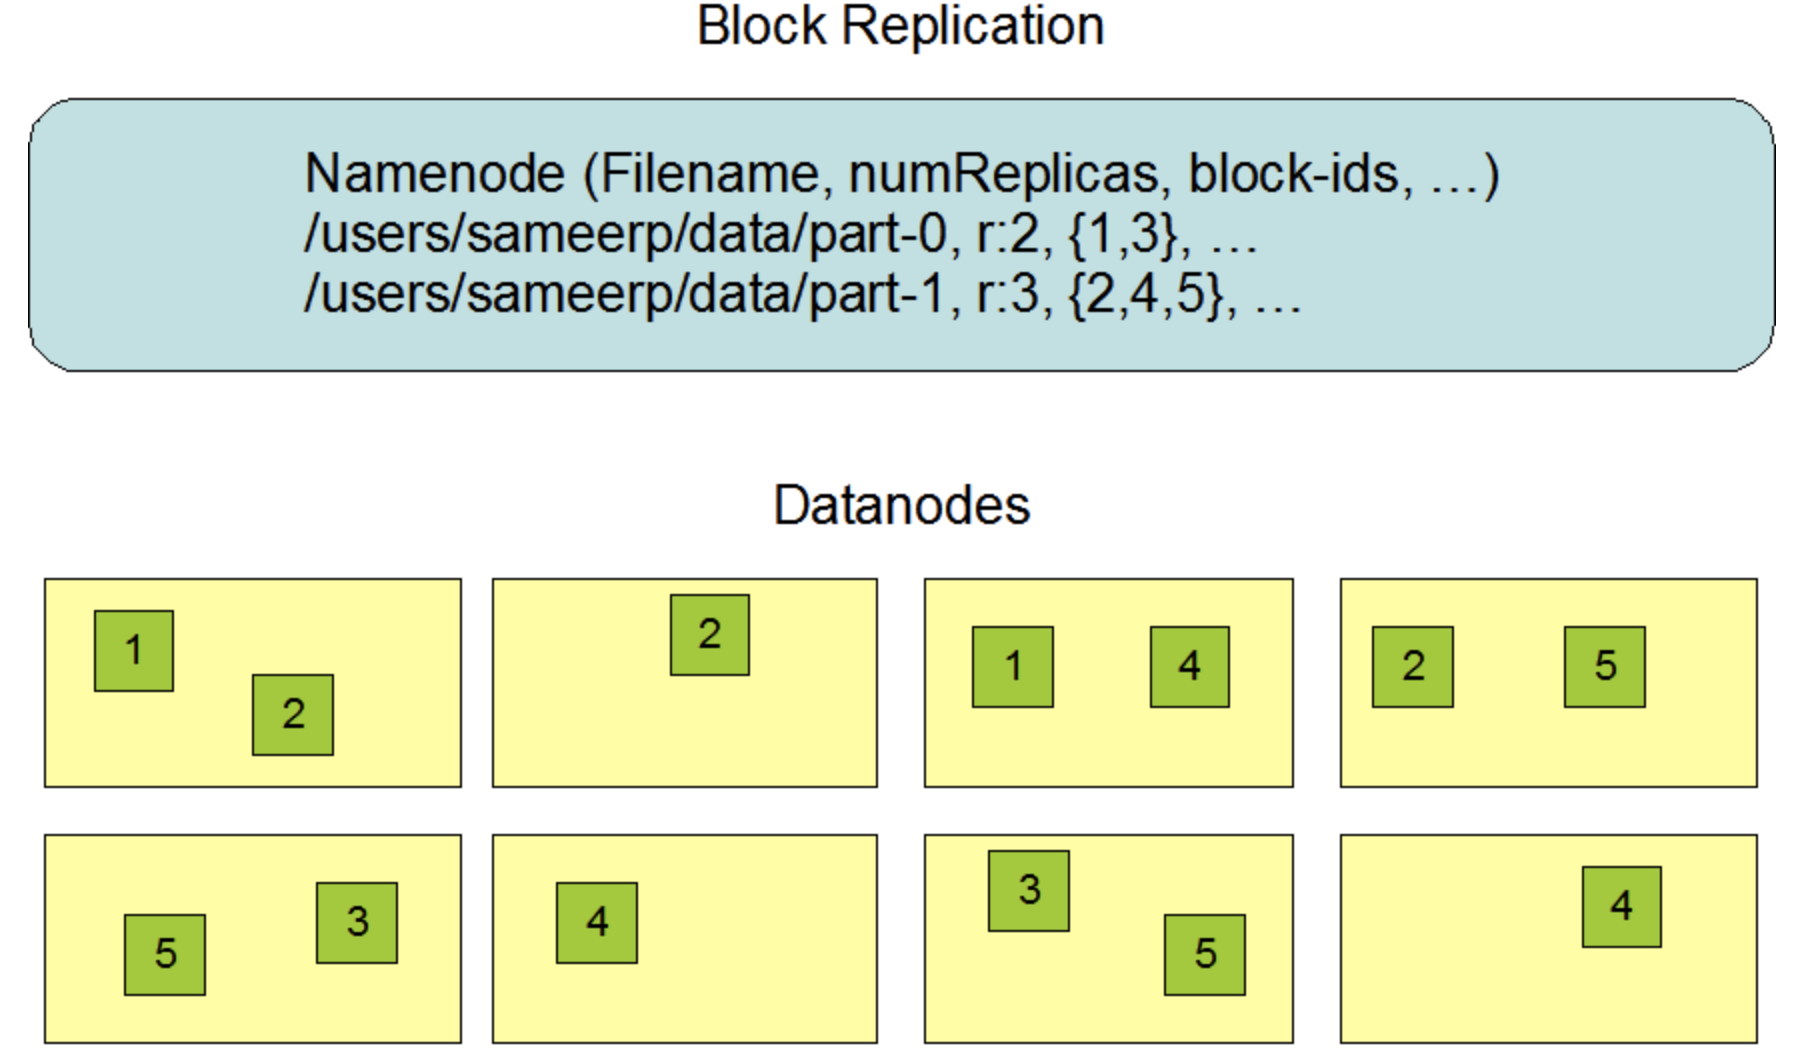
\includegraphics[height=3cm,width=0.55\columnwidth]{HDFS-replication.png}
\caption{HDFS replication system architecture~\cite{ref_url7}. A state transition adding or removing nodes maintains the total set of data.} \label{fig2}
\end{figure}

\section{Typesafe Poincare Duality}
Up until now we have not explicitly defined functoral group homomorphisms that can construct the complexes described above. We show that the dual nature of the hylomorphic and metamorphic recursion schemes maintain vanishing differentials and thus Poincare duality for all $\pi$.

If we define a catamorphism and anamorphism with the same f-algebra and f-coalgebra, we can show by construction that the resulting co/chain-complexes are valid definitions of Protocol Topologies/Manifolds and that Poincare duality of the protocol manifold is maintained up to $\pi$ isomorphism. We define in terms of $\Sigma$ and $\epsilon$, noting that our functor $\Sigma$ is a valid f-algebra and sheaf $\epsilon$ a co-algebra.

Let us define a hylomorphism
\begin{equation}
\epsilon \leftarrow P \times \Sigma  : \Omega^T(\epsilon, P)
\end{equation}
and metamorphism
\begin{equation}
\Omega_\Gamma(P, \epsilon):\Gamma_\Sigma \times \epsilon \rightarrow P  
\end{equation} 
we formally verify by the construction of the following geometric cw-complex
\begin{equation}
\Omega^T_\Gamma: 0 \xleftrightarrow{\partial} \Omega^{T^*}_{\Gamma^*}(\epsilon) \xleftrightarrow{\partial} \Omega^T_\Gamma (\epsilon(P_0)) \dots \Omega^T_\Gamma (\epsilon(P_\pi))
\end{equation}
that $T$ and $\Gamma$ form a Poincare complex, clearly satisfying the Poincare duality as $\partial$ vanishes in our construction of $T$ and $\Gamma^\epsilon_\Sigma$. The fundamental class of our corresponding space is $\Omega^{T^*}_{\Gamma^*}$ which carries the type signatures of our hylo and metamorphisms. Formally define $\Omega^{T}_{\Gamma}$ as a Poincare protocol.

\subsection{Applications: MapReduce APIs}
The design of tools in the data engineering and data science space often employ principles from functional programming and type theory due to the benefits they have at verifying code at compile time. Network queries can be implemented with guarantees around correct access governed at the type level, as functoral operators such as .map() and .reduce(). This is largely a source of the origins of scalable data processing tools for analysis and modeling like Hadoop and Spark. Distributed data stores and microservice architectures employ monadic design patterns for improvements on concurrency, static type checking, testing, design patterns, cluster management, training models etc. One benefit is the development of convenient API's with Map/Reduce operations simplifying queries by abstracting low level data locality management~\cite{ref_book2}, a key example would be Spark's RDD~\cite{ref_url1}. Monadic execution models allow complex data pipelines (see Fig.~\ref{fig3}) to be implemented and governed declaratively, providing distributed data stores constructed with high level API's. As such, if we follow their construction at the type level in architecture and code design we can develop increasingly complex distributed systems with greater guarantees.
\begin{figure}
\centering
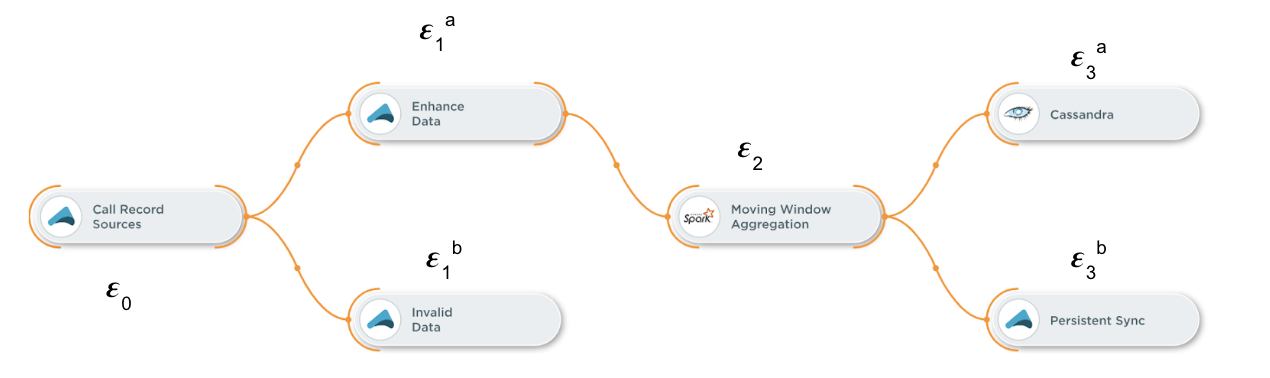
\includegraphics[height=1.7cm,width=0.55\columnwidth]{data-pipeline.png}
\caption{Example of a data pipeline with a micro-service architecture. $\epsilon$ corresponds to indices within a Poincare Complex for each micro-service.} \label{fig3}
\end{figure}
A Poincare Protocol is a consensus protocol with a monadic execution model like the Big Data tools discussed above. It describes a distributed data store of topological data formed of configuration data across blocks. An example of this is the Constellation protocol, the design of which is also its origin. Constellation was designed with a monadic execution model~\cite{ref_url6} that can be layered like a Protocol Topology and has the consistency guarantees of a Protocol Manifold. In this model, multiple independent consensus operations can coexist across heterogeneous data types, allowing for complex queries to be performed across concurrent or composite services, like common data pipelines (see Fig.~\ref{fig3}). Each of these consensus operations is referred to as a state channel, an operates on its own corresponding data type $\epsilon$. By constructing a Poincare Protocol, Constellation defined a high level MapReduce API~\cite{ref_url3} for constructing new state channels out of API callbacks across existing state channels (see Fig.~\ref{fig4}). Using an algebraic representation of these APIs in the callback tree, common in functional programming~\cite{ref_book3}, each step in the call back tree is governed by the respective $\epsilon$'s f-algebra and f-coalgebra and we can verify correctness at the type level both at compile time and runtime. The end result is a consensus protocol with the same model and guarantees of the functional programming paradigm, allowing for interoperability between the Blockchain and Big Data ecosystems. 
\begin{figure}
\centering
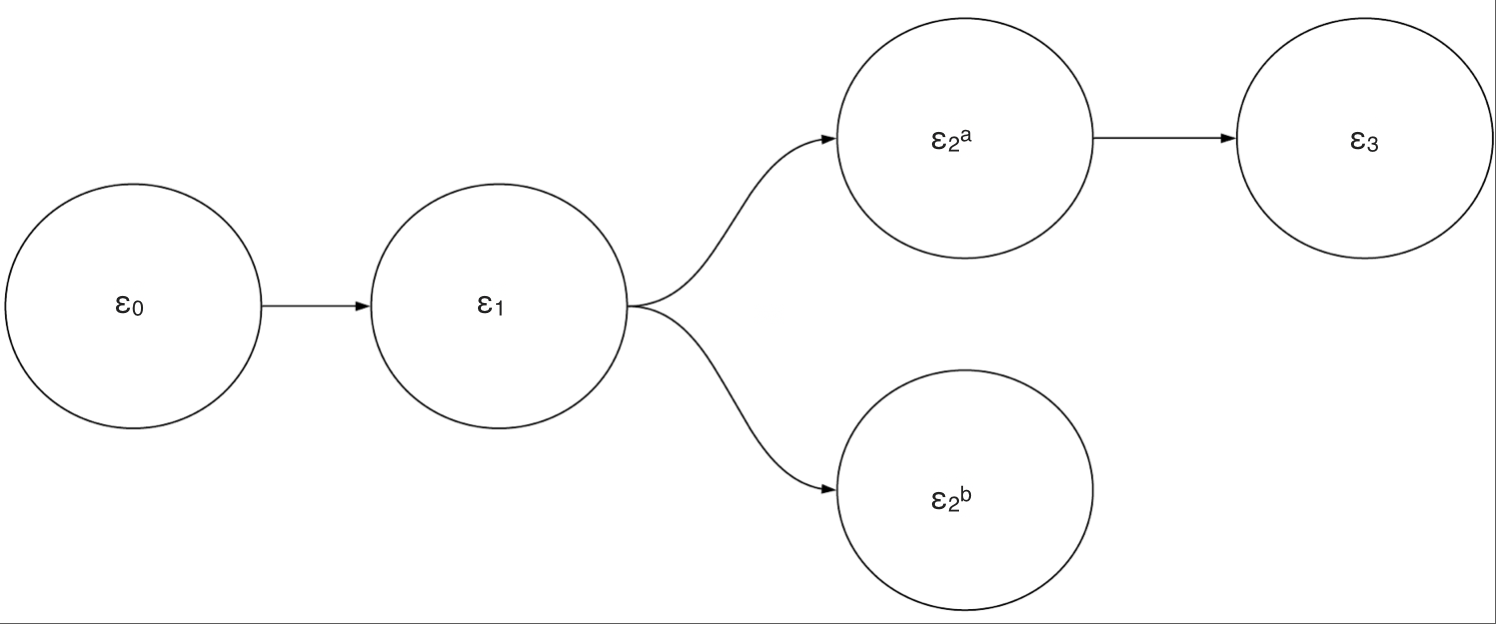
\includegraphics[height=2cm,width=0.4\columnwidth]{rec_tree_wide.png}
\caption{Callback tree across Constellation state channels (denoted by their $\epsilon$, indices within a Poincare Complex. The tree is defined by algebra/coalgebra of a recursion scheme and is transitively its own state channel.} \label{fig4}
\end{figure}
\section{Remarks} 
We have successfully constructed topological models of scalability focused Blockchain technologies and Big Data architectures. The protocol models above can be expanded to other distributed systems that undergo finite state transitions. The key advantage of these models is that they can be designed within functional languages with strong type systems that allows for verification at compile time. Future work can apply these models to systems undergoing more complex and possibly differentiable state transitions.
%
% ---- Bibliography ----
%
% BibTeX users should specify bibliography style 'splncs04'.
% References will then be sorted and formatted in the correct style.
%
\bibliographystyle{splncs04}
\bibliography{mybibliography}
%
\begin{thebibliography}{8}
\bibitem{ref_article1}
Nowak T., Schmid U.: Topology in Distributed Computing, Master's Thesis, Vienna University of Technology, (2010)

\bibitem{ref_article2}
Herlihy M., Rajsbaum S.: Algebraic topology and distributed computing a primer. In: van Leeuwen J. (eds) Computer Science Today. Lecture Notes in Computer Science, vol 1000. Springer, Berlin, Heidelberg. (1995)

\bibitem{ref_article3}
Alpern, B., Schneider F.: Defining liveness. Information Processing Letters 21, 4 (October 1985), 181--185. Cornell University, (1985)

\bibitem{ref_article4}
Saks, M., Zaharoglou, F.: Wait-free k-set agreement is impossible: the topology of public knowledge. SIAM J. Comput. 29(5), 1449–1483 (2000)

\bibitem{ref_article5}
Grahm R.: Synthetic Homology in Homotopy Type Theory Robert Graham. arXiv:1706.01540 (2017)

\bibitem{ref_article6}
Mallios A., Raptis I.: Finitary Cech-de Rham Cohomology: much ado without smoothness. Int.J.Theor.Phys. 41 1857-1902 (2002)

\bibitem{ref_article7}
Mallios, A.: Geometry of Vector Sheaves: An Axiomatic Approach to Differential Geometry, vols. 1-2, Kluwer Academic Publishers, Dordrecht (1998)

\bibitem{ref_article8}
Mallios, A.: On an Axiomatic Treatment of Differential Geometry via Vector Sheaves. Applications, Mathematica Japonica(International Plaza), 48, 93. (1988)

\bibitem{ref_article9}
Cavallo, E.: Synthetic cohomology in Homotopy Type Theory. Master’s thesis, Carnegie-Mellon University (2015)

\bibitem{ref_article10}
Nielson F. Nielson H. R.: Type and Effect Systems. In: Olderog ER., Steffen B. (eds) Correct System Design. Lecture Notes in Computer Science, vol 1710. Springer, Berlin, Heidelberg 114-136, (1999)

\bibitem{ref_article11}
A. Vahdat, M. Al-Fares, N. Farrington, R. N. Mysore, G. Porter, and S. Radhakrishnan, Scale-out networking in the data center, IEEE Micro, vol. 30, no. 4, pp. 29–41, \doi{10.1109/MM.2010.72}

\bibitem{ref_article12}
Herlihy M. and Shavit. N.: The asynchronous computability theorem for t-resilient tasks. In: Proceedings of the twenty-fifth annual ACM symposium on Theory of computing, STOC, (1993)
\bibitem{ref_article13}
Haber, S. and Stornetta, W.S. J. Cryptology  3: 99. \doi{10.1007/BF00196791} (1991)

\bibitem{ref_proc1}
Dean J., Ghemawat, S.: MapReduce: Simplified data processing on large clusters, In: Proc. 6th USENIX Symposium on Operating Systems Design and Implementation, OSDI 2004, San Francisco, USA, Dec. (2004)

\bibitem{ref_book1}
Gallier J., Quaintance J.: A Gentle Introduction to Homology, Cohomology, and Sheaf Cohomology. Preprint (2016)

\bibitem{ref_book2}
Wu D., Sakr S., Zhu L.: Big Data Programming Models. In: Zomaya A.Y, Sakr S. (eds) Handbook of Big Data Technologies, Springer International Publishing, AG,\doi{10.1007/978-3-319-49340-4\_2} (2017)

\bibitem{ref_book3}
Chuisano P., Bjarnason R.:Functional Programming in Scala, Manning Publications Co., Greenwich, CT, (2014)

\bibitem{ref_url1}
Apache Spark RDD documentation, \url{https://spark.apache.org/docs/latest/rdd-programming-guide.html\#resilient-distributed-datasets-rdds}. Last accessed 15 Oct (2019)

\bibitem{ref_url2}
Product operator from functional programming library Cats, \url{http://eed3si9n.com/herding-cats/Cartesian.html}. Last accessed 18 April (2019)

\bibitem{ref_url3}
Constellation Protocol repository, MapReduce interface via recursion schemes \url{https://github.com/Constellation-Labs/constellation/blob/7aeaa786d42e0194e31cd8fd0c6b99462cb63f33/src/main/scala/org/constellation/Cell.scala}. Last accessed 18 April (2019)

\bibitem{ref_url4}
The Bitcoin Lightning Network: Scalable Off-Chain Instant Payments. Joseph Poon, Thaddeus Dryja \url{https://lightning.network/lightning-network-paper.pdf} Last accessed 18 April (2019)

\bibitem{ref_url5}
The ZILLIQA Technical Whitepaper, The Zilliqa Team. \url{https://whitepaper.io/document/16/zilliqa-whitepaper} Last accessed 18 April (2019)

\bibitem{ref_url6}
Constellation Protocol repository, Validation Monad \url{https://github.com/Constellation-Labs/constellation/blob/dev/src/main/scala/org/constellation/util/Validation.scala}. Last accessed 18 April (2019)

\bibitem{ref_url7}
Hadoop Distributed File System design documentation \url{https://hadoop.apache.org/docs/r1.2.1/hdfs\_design.html} Last accessed 18 April (2019) 

\end{thebibliography}
\end{document}
